\Chapter{PREMIER PASSAGE EN DIFFUSION PURE}\label{sec:FPT_Diffusion}

Cette partie du mémoire est consacrée à la résolution analytique des problèmes de premier passage appliqués au processus \acl{CIR} en diffusion pure.

\section{Fonction Génératrice des Moments}\label{section_fgm_eq}
\subsection{Résolution du problème}
\paragraph{Dérivation de l'équation à résoudre}\phantom{}\\
Soit un processus d'Itô défini par l'\ac{EDS} (\ref{ito_eq}).
Il est connu que la \acl{FGM} d'un temps de premier passage $\tau(x)$ satisfait l'équation du passé de Kolmogorov (voir~\cite{cox2017} ou~\cite{lefebvre2007}): 
\[
\frac{1}{2}\sigma{(t,x)}^2M''(x;\alpha)+\mu(t,x)M'(x;\alpha)-\alpha M(x;\alpha)=0
\]
avec $M(0;\alpha)=M(c;\alpha)=1$. 

En reprenant les termes de dérive et de diffusion du \acs{CIR} (\ref{cir_eq}), l'\ac{EDO} linéaire de second ordre à résoudre devient: 
\begin{equation}\label{ode_fgm}
    \frac{1}{2}\sigma^2xM''(x;\alpha)+a(b-x)M'(x;\alpha)-\alpha M(x;\alpha)=0
\end{equation}

\paragraph{Résolution}\phantom{}\\
D'abord, en multipliant les deux côtés par $2/\sigma^2$ l'équation ci-dessus (\ref{ode_fgm}) est mise sous forme canonique: 
\[
xM''(x;\alpha)-\left(\frac{2a}{\sigma^2}x-\frac{2ab}{\sigma^2}\right)M'(x;\alpha)-\frac{2\alpha}{\sigma^2} M(x;\alpha)=0
\]
Ensuite, un changement de variable $y=\beta x$ avec $M(x;\alpha)=G(y;\alpha)$ est introduit. L'équation devient: 
\[
yG''(y;\alpha)-\left(\frac{2a}{\sigma^2} \beta y - \frac{2ab}{\sigma^2}\right)G'(y;\alpha)-\beta\frac{2\alpha}{\sigma^2} G(y;\alpha) = 0
\]
Ce changement de variable a pour objectif de déterminer, en fonction des autres paramètres du problème, la valeur de $\beta$ qui permet de ramener l'équation à la forme générale de l'équation de Kummer (\ref{kummer_eq}): 
\begin{equation}\label{kummer_eq}
    xf''(x)-(x-\theta)f'(x)-s f(x)=0,\quad\quad \theta,s\in\mathds{R}
\end{equation}
dont la solution est connue. Pour ce faire, il faut que:
\[
\frac{2a}{\sigma^2} \beta=1\implies\beta=\frac{\sigma^2}{2a}
\]
L'équation devient:
\begin{equation}\label{kummer_eq2}
    yG''(y;\alpha)-\left(y-\frac{2ab}{\sigma^2}\right)G'(y;\alpha)-\frac{\alpha}{a}G(y;\alpha) = 0
\end{equation}
La solution générale de cette dernière (\ref{kummer_eq2}) est de la forme (voir~\cite{magnus1966}): 
\[G(y;\alpha) = C_1\Phi\left(\frac{\alpha}{a}, \frac{2ab}{\sigma^2}, y\right) + C_2\Psi\left(\frac{\alpha}{a}, \frac{2ab}{\sigma^2}, y\right)\]
avec $C_1$ et $C_2$ des constantes à déterminer, et $\Phi(\cdot, \cdot, \cdot)$ et $\Psi(\cdot, \cdot, \cdot)$ sont les fonctions hypergéométriques confluentes de première et seconde espèce (voir annexe~\ref{special_functions}).

Finalement, l'expression analytique de la \acs{FGM} de $\tau(x)$ est: 
\begin{equation}\label{sol_fgm}
    M(x;\alpha) = C_1\Phi\left(\frac{\alpha}{a}, \frac{2ab}{\sigma^2}, \frac{2ax}{\sigma^2}\right) + C_2\Psi\left(\frac{\alpha}{a}, \frac{2ab}{\sigma^2}, \frac{2ax}{\sigma^2}\right)
\end{equation}

\paragraph{Détermination des constantes}\phantom{}\\
Les conditions aux limites $M(0;\alpha)=M(c;\alpha)=1$ permettent de déterminer les deux constantes $C_1$ et $C_2$ en résolvant le système suivant:
\[
\begin{cases}
    C_1\Phi\left(\frac{\alpha}{a}, \frac{2ab}{\sigma^2}, 0\right) + C_2\Psi\left(\frac{\alpha}{a}, \frac{2ab}{\sigma^2}, 0\right) = 1 \\
C_1\Phi\left(\frac{\alpha}{a}, \frac{2ab}{\sigma^2}, \frac{2ac}{\sigma^2}\right) + C_2\Psi\left(\frac{\alpha}{a}, \frac{2ab}{\sigma^2}, \frac{2ac}{\sigma^2}\right) = 1
\end{cases}
\]
Il en découle les valeurs suivantes pour $C_1$ et $C_2$: 
\begin{equation}\label{fgm_constants}
    \begin{aligned}
        &C_1 = \frac{\Phi(\frac{\alpha}{a}, \frac{2ab}{\sigma^2}, 0)-\Psi(\frac{\alpha}{a}, \frac{2ab}{\sigma^2}, 0)}{\Phi(\frac{\alpha}{a}, \frac{2ab}{\sigma^2}, \frac{2ac}{\sigma^2})\Psi(\frac{\alpha}{a}, \frac{2ab}{\sigma^2}, 0)-\Psi(\frac{\alpha}{a}, \frac{2ab}{\sigma^2}, \frac{2ac}{\sigma^2})} \\
        &C_2 = \frac{\Phi(\frac{\alpha}{a}, \frac{2ab}{\sigma^2}, \frac{2ac}{\sigma^2})-1}{\Phi(\frac{\alpha}{a}, \frac{2ab}{\sigma^2}, \frac{2ac}{\sigma^2})\Psi(\frac{\alpha}{a}, \frac{2ab}{\sigma^2}, 0)-\Psi(\frac{\alpha}{a}, \frac{2ab}{\sigma^2}, \frac{2ac}{\sigma^2})}
    \end{aligned}
\end{equation}
\subsection{Validation de l'expression obtenue}
\paragraph{Visualisation}\phantom{}\\
Il convient de valider le comportement de la \acl{FGM} $M(x;\alpha)$ définie par (\ref{sol_fgm},~\ref{fgm_constants}). À cet effet, il faut tracer son évolution sur l'intervalle $[0, c]$ pour plusieurs valeurs du paramètre $\alpha \in \{1, 2, 5, 10\}$. Concernant les paramètres du \acs{CIR} (\ref{cir_eq}), et sauf indication contraire, les valeurs utilisées pour l'ensemble des visualisations sont:
\begin{itemize}
    \item Vitesse de retour: \(a=0.1\);
    \item Moyenne long-terme: \(b=0.9\);
    \item Volatilité infinitésimale: \(\sigma=1\).
\end{itemize}
\begin{figure}[htb]
    \centering
    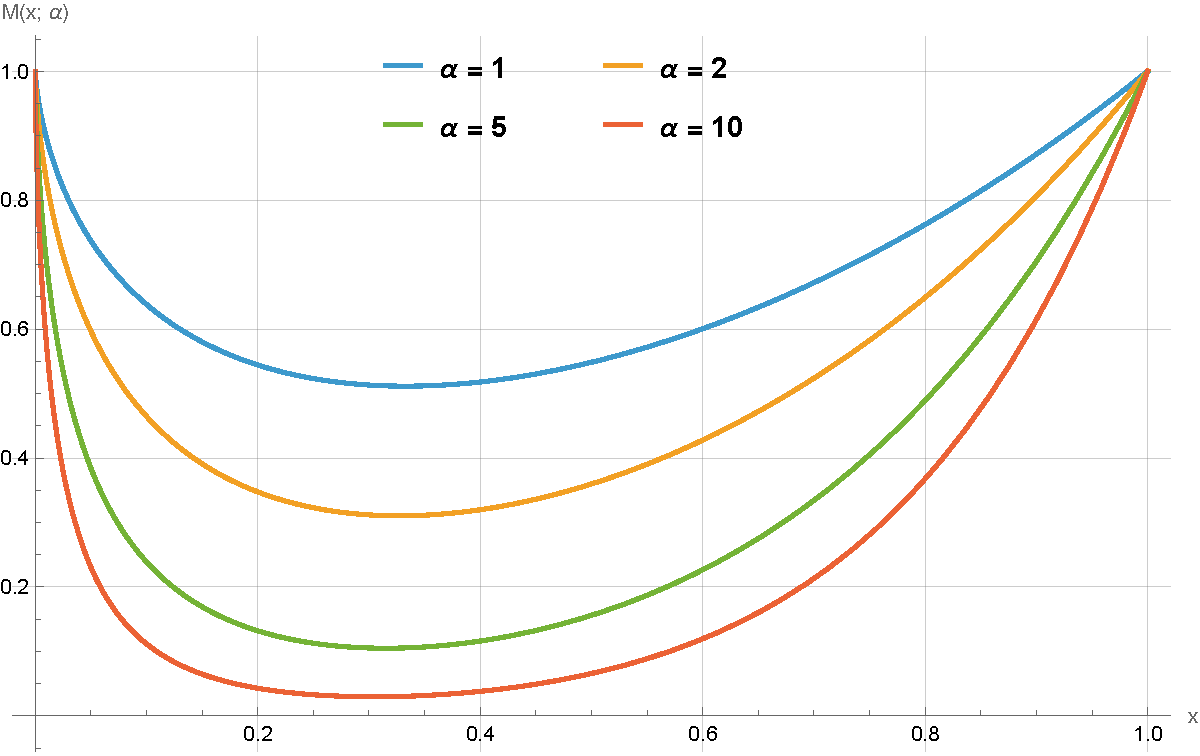
\includegraphics[width=0.5\linewidth]{img/validation/fgm.pdf}
    \caption{Visualisation de la \acl{FGM} $M(x;\alpha)$}\label{fig:FGMVisualisation}
\end{figure}
\FloatBarrier\paragraph{Analyse}\phantom{}\\
Il est important de souligner les points suivants:
\begin{itemize}
    \item Les conditions aux limites $M(0; \alpha) = M(c; \alpha) = 1$ sont respectées;
    \item Puisque $\alpha$ est par définition un paramètre positif (\ref{fgm}), la fonction est bien comprise dans l'intervalle $(0, 1)$, car elle correspond à l'exponentielle d'un nombre négatif;
    \item Par ailleurs, et pour la même raison, lorsque $\alpha$ augmente, la fonction diminue.
\end{itemize}
L'expression obtenue pour la \acl{FGM} est ainsi validée. 

\section{Fonction Temps Moyen}\label{section_mean_eq}
\subsection{Résolution du problème}
\paragraph{Dérivation de l'équation à résoudre}\phantom{}\\
En combinant le développement en série entière de l'exponentielle: 
\[
e^x=\sum_{k=0}^\infty\frac{x^k}{k!}
\]
et la définition de la \acl{FGM} (\ref{fgm}), il est possible d'écrire (en supposant que les moments de $\tau(x)$ existent et sont finis): 
\begin{equation}\label{taylor_fgm}
    \begin{aligned}
        M(x;\alpha)=\mathds{E}\left[e^{-\alpha \tau(x)}\right]&=\mathds{E}\left[\sum_{k=0}^\infty\frac{{(-\alpha\tau(x))}^k}{k!}\right] \\
        &= \sum_{k=0}^\infty\frac{{(-\alpha)}^k\mathds{E}\left[{\tau(x)}^k\right]}{k!}\\
        &=1-\alpha\mathds{E}[\tau(x)]+\frac{\alpha^2}{2}\mathds{E}\left[{\tau(x)}^2\right]-\ldots
    \end{aligned}
\end{equation}
En injectant (\ref{taylor_fgm}) dans l'équation (\ref{ode_fgm}), et en reprenant la définition (\ref{mean}), il découle l'\acs{EDO} linéaire de second ordre suivante: 
\begin{equation}\label{ode_mean}
    \frac{1}{2}\sigma^2xm''(x)+a(b-x)m'(x)=-1   
\end{equation}
avec $m(0)=m(c)=0$. En résolvant cette équation, une expression analytique de la fonction temps moyen est obtenue. 

\paragraph{Réduction d'ordre}\phantom{}\\
D'abord, afin d'alléger la notation, soit:
\begin{equation}\label{notation}
\begin{cases}
    \alpha = \frac{2a}{\sigma^2} \\
    \beta=\frac{2ab}{\sigma^2} \\
    \theta=-\frac{2}{\sigma^2}
\end{cases}
\end{equation}
L'équation peut donc être réécrite comme suit: 
\begin{equation}\label{simplified_ode_mean}
    xm''(x)+(\beta-\alpha x)m'(x)=\theta
\end{equation}
La réduction d'ordre $u(x)=m'(x)$ donne l'\acs{EDO} linéaire de premier ordre suivante:
\begin{equation}\label{order_reduction}
xu'(x)+(\beta-\alpha x)u(x)=\theta
\end{equation}
Pour procéder à sa résolution, il faut résoudre l'équation homogène associée puis déduire une solution particulière avec la méthode de variation de la constante. La solution générale obtenue est, avec $C_1$ une constante: 
\begin{equation}\label{sol_first_order_mean}
    u(x)=x^{-\beta}e^{\alpha x}(C_1-\theta \alpha^{-\beta}\Gamma(\beta, \alpha x))
\end{equation}
où $\Gamma(\cdot,\cdot)$ est la fonction Gamma incomplète (voir annexe~\ref{special_functions}).
Il suffit donc d'intégrer $u(x)$ et d'ajouter une constante $C_2$ pour obtenir l'expression de $m(x)$: 
\begin{equation}\label{intergration_sol_first_order}
    m(x)=\int u(x)dx+C_2
\end{equation}
Cependant, un problème survient lors de l'intégration du terme:
\begin{equation}\label{problematic_integral}
    \int\theta \underbrace{\phantom{|}{(\alpha x)}^{-\beta}\phantom{|}}_{P}\underbrace{\phantom{|}e^{\alpha x}\phantom{|}}_{E}\underbrace{\phantom{|}\Gamma(\beta, \alpha x)\phantom{|}}_{G}dx
\end{equation}
dans l'expression de $u(x)$ donnée par (\ref{sol_first_order_mean}). En effet, cette intégrale ne possède pas de solution analytique. Les logiciels de calcul symbolique tels que \textit{Mathematica} ou \textit{Maple} échouent également à en trouver une. Il est donc nécessaire d'explorer une autre approche afin de contourner cette difficulté.
\paragraph{Intégration}\phantom{}\\
L'intégrande de (\ref{problematic_integral}) présente des difficultés en raison de la présence du terme puissance $P:={(\alpha x)}^{-\beta}$ multiplié par le terme $E:=e^{\alpha x}$, ainsi que le terme $G:=\Gamma(\beta, \alpha x)$ (lui-même une intégrale). L'objectif est donc de reformuler cette expression afin de simplifier ou d'éliminer certains termes problématiques. C'est précisément ce qui sera abordé dans la suite de cette section. En effet, en combinant les deux expressions suivantes~\cite{NIST:DLMF}: 
\begin{align*}
    \left\{
    \begin{aligned}
        \Gamma(s,x) &= \Gamma(s)-\gamma(s,x) \\
        \gamma(s,x) &= x^s\Gamma(s)e^{-x}\sum_{k=0}^{\infty} \frac{x^k}{\Gamma(s+k+1)}
    \end{aligned}
    \right.
\end{align*}
avec $\gamma(\cdot,\cdot)$ une autre forme de la fonction gamma incomplète (voir annexe~\ref{special_functions}). 

Il est possible d'écrire:
\[
    \Gamma(s,x) = \Gamma(s)-x^s\Gamma(s)e^{-x}\sum_{k=0}^{\infty} \frac{x^k}{\Gamma(s+k+1)}
\]
et donc, en reprenant les termes de l'équation à résoudre (\ref{notation}) il découle l'expression suivante: 
\begin{equation}\label{incomplete_gamma_simplification}
    \Gamma(\beta, \alpha x) = \Gamma(\beta)-\Gamma(\beta)\underbrace{\phantom{|}{(\alpha x)}^\beta\phantom{|}}_{P'} \underbrace{\phantom{|}e^{-\alpha x}\phantom{|}}_{E'}\sum_{k=0}^{\infty} \frac{{(\alpha x)}^k}{\Gamma(\beta+k+1)}
\end{equation}
L'expression ci-dessus (\ref{incomplete_gamma_simplification}) est très intéressante. En effet, en remplaçant le terme $G$ dans (\ref{problematic_integral}) par (\ref{incomplete_gamma_simplification}), les termes $P$ et $P'$ ainsi que $E$ et $E'$ se simplifient comme suit:
\[
    \begin{aligned}
        &\int\theta \underbrace{\phantom{|}{(\alpha x)}^{-\beta}\phantom{|}}_{P}\underbrace{\phantom{|}e^{\alpha x}\phantom{|}}_{E}\overbrace{\left(\Gamma(\beta)-\Gamma(\beta)\underbrace{\phantom{|}{(\alpha x)}^\beta\phantom{|}}_{P'} \underbrace{\phantom{|}e^{-\alpha x}\phantom{|}}_{E'}\sum_{k=0}^{\infty} \frac{{(\alpha x)}^k}{\Gamma(\beta+k+1)}\right)}^{G}dx \\
        &= \int\theta\Gamma(\beta)\underbrace{\phantom{|}{(\alpha x)}^{-\beta}\phantom{|}}_{P}\underbrace{\phantom{|}e^{\alpha x}\phantom{|}}_{E}dx-\int\theta\Gamma(\beta)\underbrace{\phantom{|}{(\alpha x)}^{-\beta}\phantom{|}}_{P}\underbrace{\phantom{|}{(\alpha x)}^\beta\phantom{|}}_{P'}\underbrace{\phantom{|}e^{\alpha x}\phantom{|}}_{E} \underbrace{\phantom{|}e^{-\alpha x}\phantom{|}}_{E'}\sum_{k=0}^{\infty} \frac{{(\alpha x)}^k}{\Gamma(\beta+k+1)} \\
        &= \int\theta\Gamma(\beta)\underbrace{\phantom{|}{(\alpha x)}^{-\beta}\phantom{|}}_{P}\underbrace{\phantom{|}e^{\alpha x}\phantom{|}}_{E}dx-\theta\Gamma(\beta)\int\sum_{k=0}^{\infty} \frac{{(\alpha x)}^k}{\Gamma(\beta+k+1)}
    \end{aligned}
\]
En injectant dans (\ref{intergration_sol_first_order}), il découle: 
\[
m(x)=(C_1-\theta\alpha^{-\beta}\Gamma(\beta))\underbrace{\int x^{-\beta}e^{\alpha x}dx}_I + \,\theta\Gamma(\beta) \underbrace{\int\sum_{k=0}^{\infty} \frac{{(\alpha x)}^k}{\Gamma(\beta+k+1)}dx}_J + C_2
\]
avec $I$ et $J$ deux intégrales à résoudre: 
\begin{itemize}
    \item \textbf{Résolution de} $I$: \\
    \textit{Wolfram Mathematica} donne:
    \begin{equation}\label{exponential_integral}
        \int x^{-\beta}e^{\alpha x}dx = -x^{1-\beta}E_\beta(-\alpha x)
    \end{equation}
    où $E_n(x)$ est la fonction intégrale exponentielle généralisée (voir annexe~\ref{special_functions}).
    La relation suivante~\cite{abramowitz1964}:
    \[
    E_n(x)=x^{n-1}\Gamma(1-n,x)
    \]
    permet d'écrire: 
    \begin{equation}\label{exponential_integral_simplification}
        E_{\beta}(-\alpha x)={(-\alpha x)}^{\beta-1}\Gamma(1-\beta,-\alpha x)
    \end{equation}
    En combinant (\ref{exponential_integral}) et (\ref{exponential_integral_simplification}), l'expression analytique de la solution de $I$ est obtenue:
    \[
        I=-{(-\alpha)}^{\beta-1}\Gamma(1-\beta,-\alpha x)
    \]
    \item \textbf{Résolution de $J$}: \\
    La série à l'intérieur de l'intégrale converge uniformément grâce au terme factoriel au dénominateur. L'intégration terme-à-terme est donc possible: 
    \[
    \begin{aligned}
        \int\sum_{k=0}^{\infty} \frac{{(\alpha x)}^k}{\Gamma(\beta+k+1)}dx &= \sum_{k=0}^{\infty} \int \frac{{(\alpha x)}^k}{\Gamma(\beta+k+1)}dx \\
        &= \sum_{k=0}^{\infty} \frac{\alpha^k x^{k+1}}{(k+1)\Gamma(\beta+k+1)} \\
        &= \frac{x}{\Gamma(1+\beta)}\,_2F_2\left(\begin{bmatrix}1\\1\end{bmatrix},\begin{bmatrix}2\\1+\beta\end{bmatrix},\alpha x\right)
    \end{aligned}
    \]
    où $_p F_q(\cdot,\cdot,\cdot)$ est la fonction hypergéométrique généralisée (voir annexe~\ref{special_functions}).
    
\end{itemize}
La forme finale de l'expression de la fonction temps moyen est donc:
\begin{equation}\label{sol_mean}
    m(x)={(-\alpha)}^{\beta-1}\Gamma(1-\beta,-\alpha x)\left[\theta\alpha^{-\beta}\Gamma(\beta)-C_1\right]+\frac{\theta x}{\beta}\,{}_2F_2\left(\begin{bmatrix}1\\1\end{bmatrix},\begin{bmatrix}2\\1+\beta\end{bmatrix},\alpha x\right) + C_2
\end{equation}

\paragraph{Détermination des constantes}\phantom{}\\
Les conditions aux limites $m(0)=m(c)=0$ permettent de déterminer les deux constantes $C_1$ et $C_2$ en résolvant le système suivant: 
\begin{align*}
\left\{\begin{aligned}
(\theta\alpha^{-\beta}\Gamma(\beta)-C_1)\alpha^{\beta-1}\Gamma(1-\beta) + C_2 &= 0\\
(\theta\alpha^{-\beta}\Gamma(\beta)-C_1)\alpha^{\beta-1}\Gamma(1-\beta,\alpha c) + \frac{c\theta}{\beta}\,{}_2F_2\left(\begin{bmatrix}1\\1\end{bmatrix},\begin{bmatrix}2\\1+\beta\end{bmatrix},\alpha c\right)+ C_2 &= 0
\end{aligned}\right. \\
\end{align*}
Les expressions des constantes $C_1$ et $C_2$ sont donc:
\begin{equation}\label{mean_constants}
    \begin{aligned}
        C_1 &= \alpha^{-\beta}\theta\Gamma(\beta)+\frac{\alpha c \theta {(-\alpha)}^{-\beta}}{\beta\gamma(1-\beta,\alpha c)}\,{}_2F_2\left(\begin{bmatrix}1\\1\end{bmatrix},\begin{bmatrix}2\\1+\beta\end{bmatrix},\alpha c\right) \\
        C_2 &= -\frac{c\theta\Gamma(1-\beta)}{\beta\gamma(1-\beta,\alpha c)}\,{}_2F_2\left(\begin{bmatrix}1\\1\end{bmatrix},\begin{bmatrix}2\\1+\beta\end{bmatrix},\alpha c\right)
    \end{aligned}
\end{equation}
avec $\alpha$, $\beta$ et $\theta$ définis en (\ref{notation}).
\subsection{Validation de l'expression obtenue}

\paragraph{Visualisation}\phantom{}\\
Enfin, il est nécessaire de valider le comportement de la fonction Temps Moyen $m(x)$ définie par (\ref{sol_mean},~\ref{mean_constants}). La fonction est donc tracée pour différentes valeurs des paramètres $a,\;\forall\;a\in\{0.1,0.2,0.4\}$ et $\sigma,\;\forall\;\sigma\in\{1,\sqrt{2},2\}$.


\begin{figure}[htb]
    \centering
    \begin{subfigure}{0.45\linewidth}
        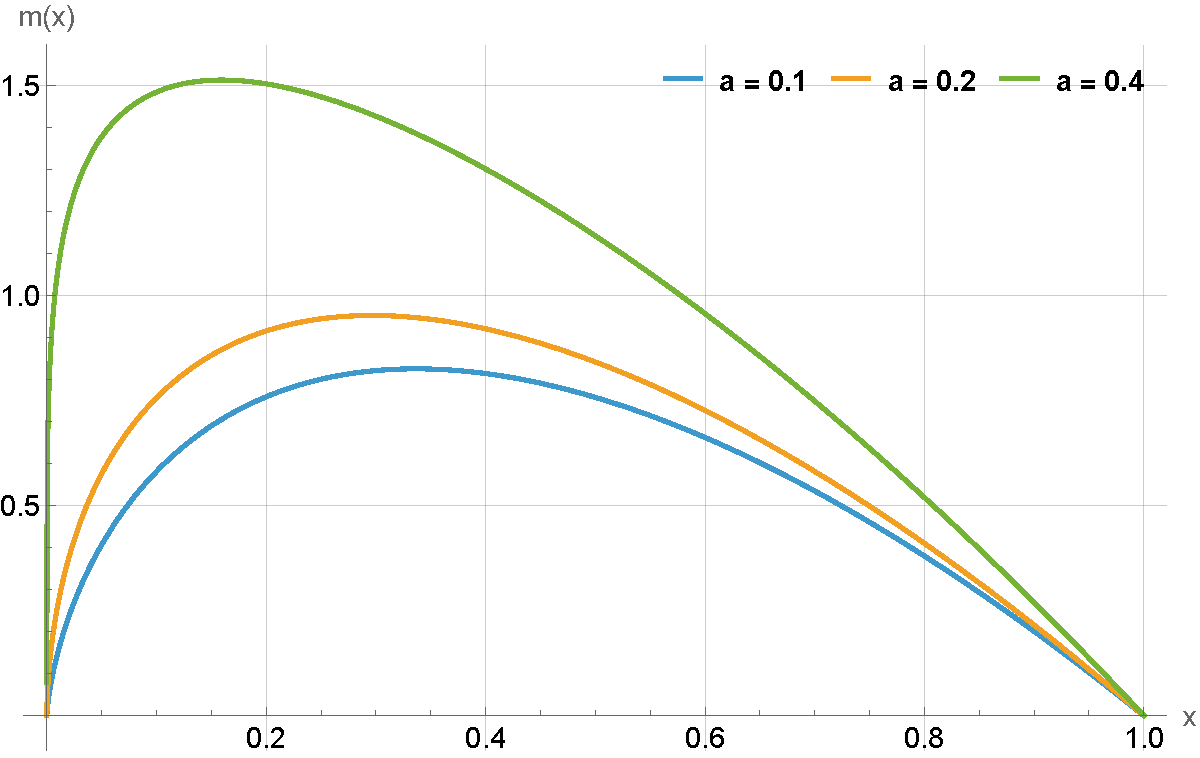
\includegraphics[width=\linewidth]{img/validation/Mean/mean_a.pdf}
        \caption{Sensibilité de la vitesse $a$}\label{fig:Mean_a_visualisation}
    \end{subfigure}
    \hfill
    \begin{subfigure}{0.45\linewidth}
        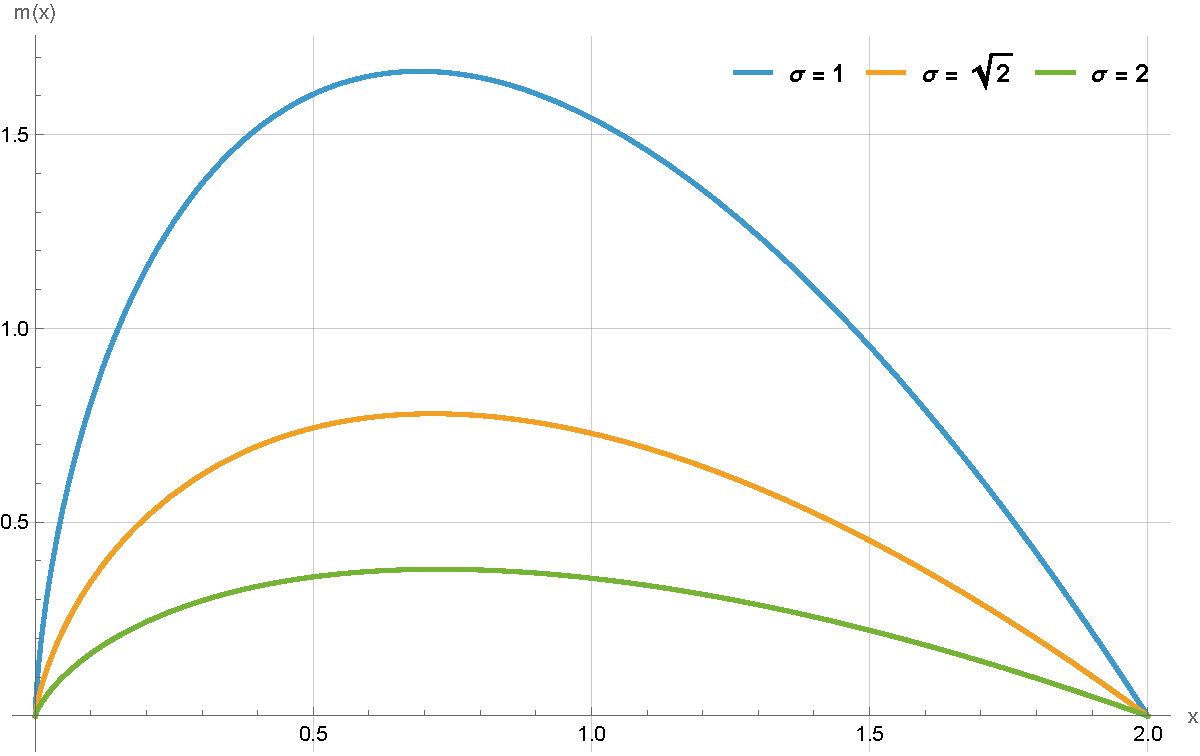
\includegraphics[width=\linewidth]{img/validation/Mean/mean_sigma.pdf}
        \caption{Sensibilité de la volatilité infinitésimale $\sigma$}\label{fig:Mean_sigma_visualisation}
    \end{subfigure}
    \caption{Visualisation de la fonction Temps Moyen $m(x)$}\label{fig:MeanVisualisation}
\end{figure}
\FloatBarrier\paragraph{Analyse}\phantom{}\\
Il est important de noter les points suivants:
\begin{itemize}
    \item Les conditions aux limites $m(0)=m(c)=0$ sont respectées;
    \item Cette fonction représente un \textit{temps moyen de premier passage}, elle doit donc être positive pour toute valeur de $x$ dans $[0,c]$;
    \item Une augmentation de la vitesse de retour $a$ entraîne une hausse du temps moyen de sortie de l'intervalle. En effet, plus la force de rappel vers la moyenne est forte (i.e., $a$ élevé), plus une déviation significative et peu probable est nécessaire pour franchir les bornes de l'intervalle;
    \item À l'inverse, une augmentation de la volatilité infinitésimale $\sigma$ diminue le temps moyen de sortie. Cela s'explique naturellement: des fluctuations plus intenses accroissent la probabilité de quitter rapidement l'intervalle.
\end{itemize}

L'expression obtenue pour la fonction de temps moyen de premier passage est ainsi validée.

\section{Fonction Aire Moyenne}
\subsection{Résolution du problème}
\paragraph{Dérivation de l'équation à résoudre}\phantom{}\\
Il est connu que l'\acs{EDO} de second ordre régissant la fonction (\ref{area}) est (voir~\cite{abundo2013}): 
\[\frac{1}{2}\sigma^2xA''(x)+a(b-x)A'(x)=-x\]
En reprenant les notations introduites en (\ref{notation}), l'équation devient: 
\[xA''(x)+(\beta-\alpha x)A'(x)=\theta x\]
Il convient de noter que cette équation ressemble beaucoup à celle dérivée en (\ref{simplified_ode_mean}). La résolution se fera donc de manière semblable.
\paragraph{Réduction d'ordre}\phantom{}\\
En procédant de façon identique à la résolution de l'équation du temps moyen (\ref{order_reduction},~\ref{sol_first_order_mean},~\ref{intergration_sol_first_order}), il est possible d'écrire: 
\[xu'(x)+(\beta-\alpha x)u(x)=\theta x\]
et donc: 
\[u(x)=C_1x^{-\beta} e^{\alpha x} -\theta\alpha^{-\beta-1}x^{-\beta} e^{\alpha x}\Gamma(\beta+1, \alpha x)\]
En combinant l'expression dérivée précédemment (\ref{incomplete_gamma_simplification}) et l'identité suivante~\cite{NIST:DLMF}: 
\[\Gamma(s+1, x)=s\Gamma(s, x)+x^s e^{-x}\]
il est possible de réécrire la solution sous la forme: 
\[
u(x)=C_1x^{-\beta} e^{\alpha x} -\theta\alpha^{-\beta-1}\left(\beta x^{-\beta}e^{\alpha x}\Gamma(\beta)\left(1-{(\alpha x)}^\beta e^{-\alpha x}\sum_{k=0}^{\infty} \frac{{(\alpha x)}^k}{\Gamma(\beta+k+1)}\right)+1\right)
\]

\paragraph{Intégration}\phantom{}\\
Pour obtenir la forme explicite de $A(x)$, il suffit d'intégrer $u(x)$ et d'ajouter une deuxième constante:
\[
\begin{aligned}
    A(x) &= \int u(x)dx+C_2 \\
    &= (C_1-\theta\alpha^{-\beta-1}\Gamma(\beta+1))\underbrace{\int x^{-\beta}e^{\alpha x}dx}_I +\frac{\theta\beta\Gamma(\beta)}{\alpha}\underbrace{\int\sum_{k=0}^{\infty} \frac{{(\alpha x)}^k}{\Gamma(\beta+k+1)}dx}_J-\theta\alpha^{-\beta-1}x +C_2 \\
\end{aligned}
\]
Les deux intégrales résolues précédemment $I$ et $J$ réapparaissent. En injectant leurs solutions analytiques, la forme finale de l'expression de la fonction Aire Moyenne est obtenue: 
\begin{equation}\label{sol_area}
    \begin{aligned}
            A(x) = {(-\alpha)}^{\beta-1}\Gamma(1-\beta,-\alpha x)[\theta\alpha^{-\beta-1}\Gamma(\beta+1)-C_1]\\+\frac{x\theta}{\alpha}\left[{}_2F_2\left(\begin{bmatrix}1\\1\end{bmatrix},\begin{bmatrix}2\\1+\beta\end{bmatrix},\alpha x\right)-\alpha^{-\beta}\right] +C_2 
    \end{aligned}
\end{equation}


\paragraph{Détermination des constantes}\phantom{}\\
Les conditions aux limites $A(0)=A(c)=0$ nous permettent de déterminer les deux constantes $C_1$ et $C_2$ en résolvant le système suivant: 
\begin{align*}
\left\{\begin{aligned}
    {(-\alpha)}^{\beta-1}\Gamma(1-\beta)(\theta\alpha^{-\beta-1}\Gamma(\beta+1)-C_1)+C_2 &= 0 \\
    {(-\alpha)}^{\beta-1}\Gamma(1-\beta,-\alpha c)[\theta\alpha^{-\beta-1}\Gamma(\beta+1)-C_1]\\+ \frac{c\theta}{\alpha}\left[{}_2F_2\left(\begin{bmatrix}1\\1\end{bmatrix},\begin{bmatrix}2\\1+\beta\end{bmatrix},\alpha c\right)-\alpha^{-\beta}\right] +C_2 &=0
\end{aligned}\right.
\end{align*}
Les constantes $C_1$ et $C_2$ s'écrivent donc: 
\begin{equation}\label{area_constants}
    \begin{aligned}
        C_1 =& \frac{1}{\gamma (1-\beta ,-\alpha c)}\Bigg[\theta  {(-\alpha)}^{-\beta } \alpha ^{-\beta -1} \Bigg\{c \alpha ^{\beta +1} \,{}_2F_2\left(\begin{bmatrix}1\\1\end{bmatrix},\begin{bmatrix}2\\1+\beta\end{bmatrix},\alpha c\right)\\&\quad\quad\quad\quad\quad\quad\quad\quad\quad\quad+
        {(-\alpha)}^{\beta } \Gamma(\beta +1)\gamma (1-\beta ,-c \alpha )-\alpha  c\Bigg\}\Bigg] \\
        C_2 =& -\frac{c \theta  \alpha ^{-\beta -1} \Gamma (1-\beta ) }{\gamma(1-\beta ,-c \alpha )}\left[\alpha ^{\beta } \,{}_2F_2\left(\begin{bmatrix}1\\1\end{bmatrix},\begin{bmatrix}2\\1+\beta\end{bmatrix},\alpha c\right)-1\right]
    \end{aligned}
\end{equation}

\subsection{Validation de l'expression obtenue}
\paragraph{Visualisation}\phantom{}\\
Par ailleurs, la même démarche de validation est effectuée pour la fonction Aire Moyenne $A(x)$ définie par (\ref{sol_area},~\ref{area_constants}).

\begin{figure}[htb]
    \centering
    \begin{subfigure}{0.45\linewidth}
        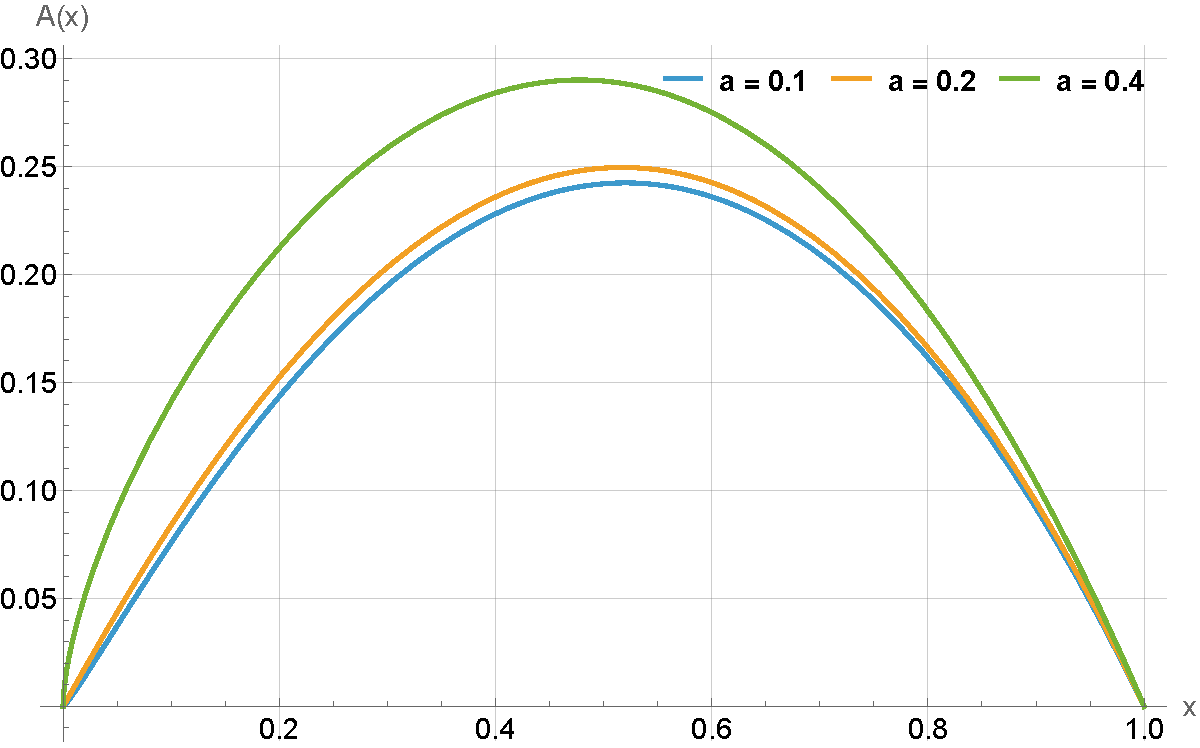
\includegraphics[width=\linewidth]{img/validation/Area/area_a.pdf}
        \caption{Sensibilité de la vitesse $a$}\label{fig:Area_a_visualisation}
    \end{subfigure}
    \hfill
    \begin{subfigure}{0.45\linewidth}
        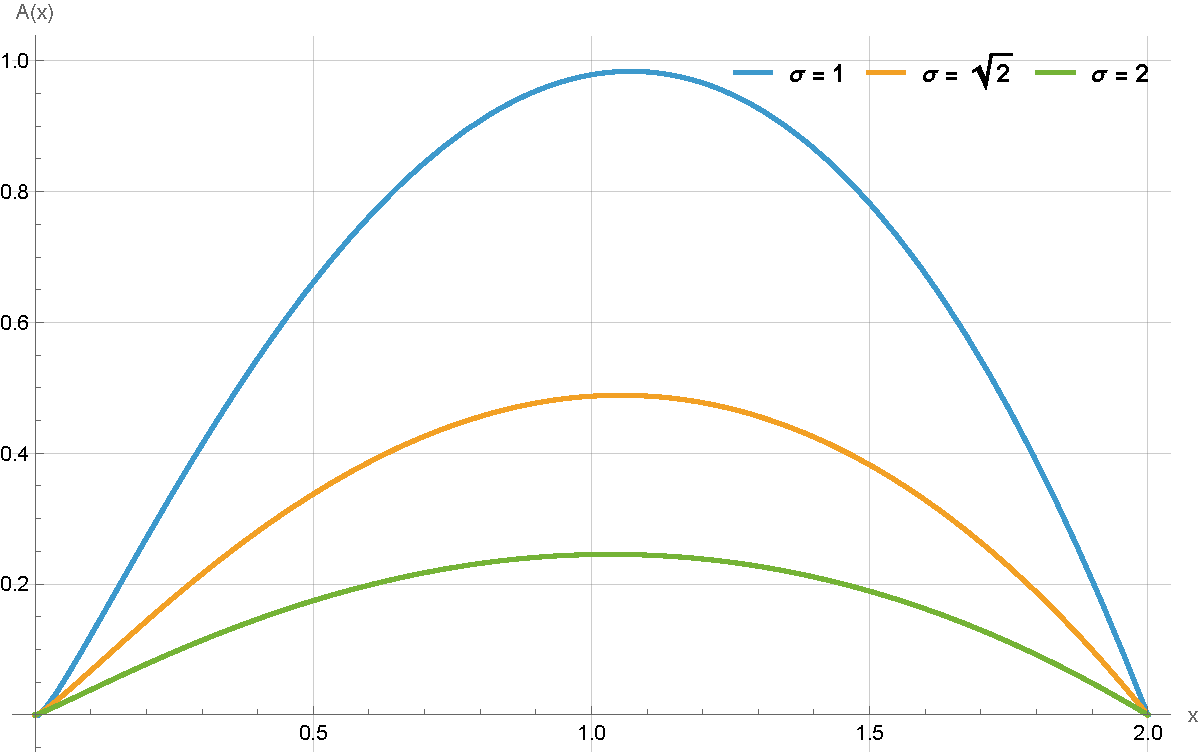
\includegraphics[width=\linewidth]{img/validation/Area/area_sigma.pdf}
        \caption{Sensibilité de la volatilité infinitésimale $\sigma$}\label{fig:Area_sigma_visualisation}
    \end{subfigure}
    \caption{Visualisation de la fonction Aire Moyenne $A(x)$}\label{fig:AreaVisualisation}
\end{figure}
\FloatBarrier\paragraph{Analyse}\phantom{}\\
Il convient de souligner les points suivants:
\begin{itemize}
    \item Les conditions aux limites $A(0)=A(c)=0$ sont respectées;
    \item Cette fonction représente une \textit{aire moyenne} sous un processus positif, elle doit donc être positive pour toute valeur de $x$ dans $[0,c]$;
    \item Une augmentation de la vitesse de retour $a$ entraîne une augmentation de l'aire moyenne sous le processus avant la sortie de l'intervalle. En effet, une force de rappel plus intense maintient le processus autour de sa moyenne plus longtemps, retardant la sortie et augmentant ainsi l'accumulation totale;
    \item À l'inverse, une augmentation de la volatilité infinitésimale $\sigma$ réduit l'aire moyenne. Des fluctuations plus fortes rendent les sorties plus précoces, limitant la durée pendant laquelle le processus peut contribuer à l'intégrale.
\end{itemize}

L'expression obtenue pour la fonction Aire Moyenne est ainsi validée.
